\section{Measurements}

\subsection{RRC State Inference}
The previous RRC state inference study provides a decent methodology to infer the RRC state machines~\cite{3g_rrc}. They want to infer the DCH demotion timer and FACH demotion timer in the RRC state machine. The methodology is to send a MAX (1024) bytes size packets to let the handset promote to DCH. Then wait for various amount of times (or called gap periods) to allow the handset stay in DCH, or demote to FACH, or even further demote to PCH. And send another packet with size of Max or Min (30) bytes. They measure the RTT (Round Trip Time) delay for each fixed gap period. They will infer the demotion timer by observing a larger RTT difference between two consecutive pre-defined gap periods. For example, if the RTT at gap period of 4 s is 3 times larger than that of 3.5 s, then they will conclude the FACH demotion timer is around 4 s. Since the handset will demote to FACH and promote to DCH (sending another packet) again at 4 s, the extra state transition delay contributes to the larger RTT. I repeat their experiments using UDP packets, and let the server respond an echo packets once the transmitted packet get received. In Figure~\ref{fig:rrc.infer}, I could observe an unexpected delay over FACH initial state and FACH to DCH promotion transitions, which implies the latency that mobile user could experience during the initial stage of data transmission.

% RLC Loss ratio per RRC state
\begin{figure}
\centering
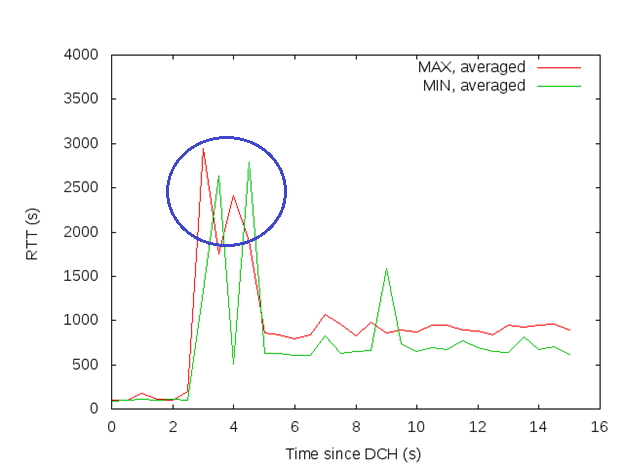
\includegraphics[width=0.45\textwidth]{figs/rrc_infer.png}
\caption{Unexpected large RTT during initial part of FACH state and FACH to DCH promotion transition}
\label{fig:rrc.infer}
\end{figure}

\subsection{Control Experiments}

% UDP/ TCP control experiment set up
The purpose of the control experiments is to verify the unexpected delays over noisy FACH state, and identify the root cause of the problem. First, we repeated our active RRC inference test for 160+ hours and dump both the client QxDM and server side tcpdump traces to perform offline analysis~\cite{tcpdump}. In order to distinguish the identities of each UDP packets, we manually injected a "sequence number" into the first four bytes of the sender's randomized payload, and the echo server sent back the received sequence number as acknowledge number in its payload. I refer the trace as \emph{UDP\_{}Trace}. Second, we designed a packet train probing using TCP packets so that we could recreate the "pseudo-state" issue~\cite{pkt.train}. Basically, we send a "train" of TCP packet size of 10 KB bytes with interleaving gap period of 3 seconds to 5 seconds incremented by 0.5 seconds with the total of 500 packets. The gap period is the DCH demotion timer period considering the variance in the lossy channel, and adjacent packet will transmit the packet starting from FACH state. Therefore, we will have more transition over the troublesome FACH state to allow us to take a closer look the root cause. Since TCP has its own ARQ (automatic repeat request) mechanism, it would be interesting to investigate the RLC retransmission's delay influence over TCP retransmission. I will refer the trace as \emph{TCP\_{}Trace}.

\label{sec:measure}

